\documentclass[11pt,letterpaper]{article}
\usepackage[lmargin=1in,rmargin=1in,tmargin=1in,bmargin=1in]{geometry}
\usepackage{../style/homework}
\usepackage{../style/commands}
\setbool{quotetype}{true} % True: Side; False: Under
\setbool{hideans}{false} % Student: True; Instructor: False

% -------------------
% Content
% -------------------
\begin{document}

\homework{10: Due 10/30}{The study of mathematics, like the Nile, begins in minuteness but ends in magnificence.}{Charles Caleb Colton}

% Problem 1
\problem{10} Consider the relation $f$ plotted below. 
	\[
	\fbox{
	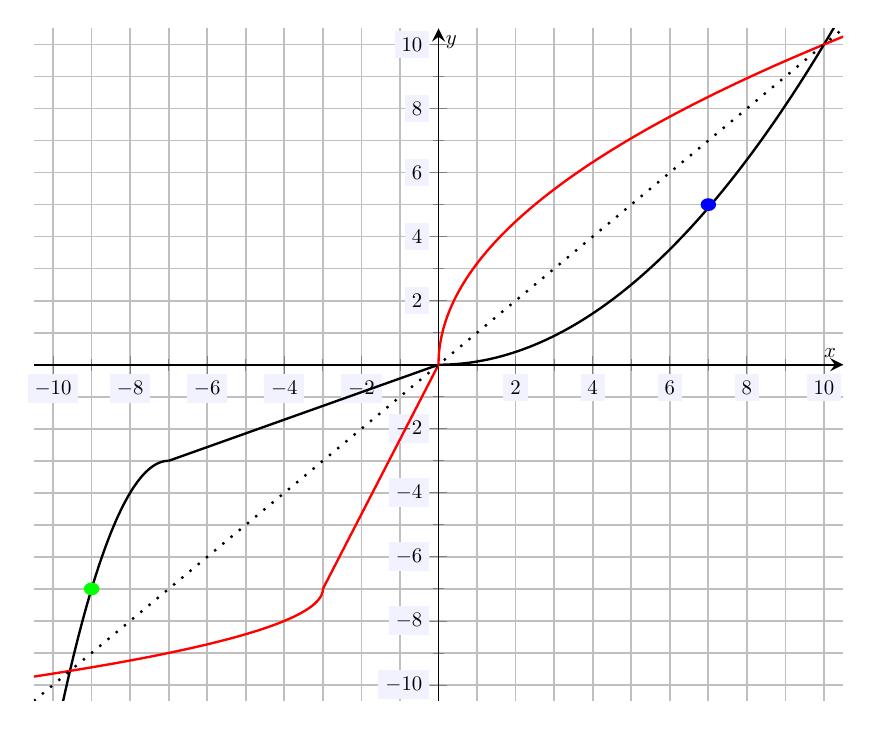
\begin{tikzpicture}[scale=1.5,every node/.style={scale=0.5}]
	\begin{axis}[
	grid=both,
	axis lines=middle,
	ticklabel style={fill=blue!5!white},
	xmin= -10.5, xmax=10.5,
	ymin= -10.5, ymax=10.5,
	xtick={-10,-8,-6,-4,-2,0,2,4,6,8,10},
	ytick={-10,-8,-6,-4,-2,0,2,4,6,8,10},
	minor tick = {-10,-9,...,10},
	xlabel=\(x\),ylabel=\(y\),
	]
	\addplot[line width= 0.02cm,samples=100,domain= -10.5:-7] ({x},{-(x + 7)^2 - 3}); 
	\addplot[line width= 0.02cm,samples=100,domain= -7:0] ({x},{3/7*x}); 
	\addplot[line width= 0.02cm,samples=100,domain= 0:10.5] ({x},{x^2/10}); 
	
	\draw[fill=blue,draw=none] (7,5) circle (0.2);
	\draw[fill=green,draw=none] (-9,-7) circle (0.2);

	\addplot[line width= 0.02cm,samples=100,domain= -10.5:-7,red] ({-(x + 7)^2 - 3},{x}); 
	\addplot[line width= 0.02cm,samples=100,domain= -7:0,red] ({3/7*x},{x}); 
	\addplot[line width= 0.02cm,samples=100,domain= 0:10.5,red] ({x^2/10},{x}); 	
	
	\addplot[line width= 0.02cm,samples=100,domain= -10.5:10.5,dotted] ({x},{x}); 
	\end{axis}
	\end{tikzpicture}
	}
	\] 

\begin{enumerate}[(a)]
\item Compute $f(7)$ and $f(-9)$. 
\item Is $f(x)$ a function? Explain. 
\item Does $f(x)$ have an inverse? If so, sketch the inverse. If not, explain why. 
\end{enumerate} \pspace

\sol 
\begin{enumerate}[(a)]
\item Because the plot contains the points $(7, 5)$ and $(-9, -7)$, shown in plot above in blue and green, respectively, we can see that $f(7)= 5$ and $f(-9)= -7$. \pspace

\item Yes, $f(x)$ is a function because it passes the vertical line test; that is, every vertical line intersects the relation at most once. \pspace

\item Yes, the function $f(x)$ has an inverse because it passes the horizontal line test; that is, every horizontal line intersects the function at most once. We know that the graph of the inverse function for $f(x)$ is the reflection of $f(x)$ through the line $y= x$. We sketch this above in red. The line $y= x$ is sketched as a dotted black line. 
\end{enumerate}



\newpage



% Problem 2
\problem{10} Showing all your work, verify that $g(x)= 4x + 9$ is the inverse function for $f(x)= \frac{x - 9}{4}$. Also, compute $g(-2)$. What does the value of $g(-2)$ tell you about the function $f(x)$? \pspace

\sol We know that $g= f^{-1}$ if $(f \circ g)(x)= x$ and $(g \circ f)(x)= x$. We verify this:
	\[
	\begin{aligned}
	(f \circ g)(x)&= f \big( g(x) \big) &\qquad\qquad (g \circ f)(x)&= g\big( f(x) \big) \\
	&=f(4x + 9) & &= g \left( \dfrac{x - 9}{4} \right) \\
	&= \dfrac{(4x + 9) - 9}{4} & &= 4 \left( \dfrac{x - 9}{4} \right) + 9 \\
	&= \dfrac{4x}{4} & &= (x - 9) + 9 \\
	&= x & &= x
	\end{aligned}
	\]
Therefore, $g$ is the inverse of $f$, i.e. $g= f^{-1}$. \pspace

We have\dots
	\[
	g(-2)= 4(-2) + 9= -8 + 9= 1
	\] \pspace
Of course, because $g= f^{-1}$, this tells us that $f^{-1}(-2)= 1$, i.e. $f(1)= -2$. We can verify this:
	\[
	f(1)= \dfrac{1 - 9}{4}= \dfrac{-8}{4}= -2
	\]



\newpage



% Problem 3
\problem{10} A relation $\phi$ is plotted below. 
	\[
	\fbox{
	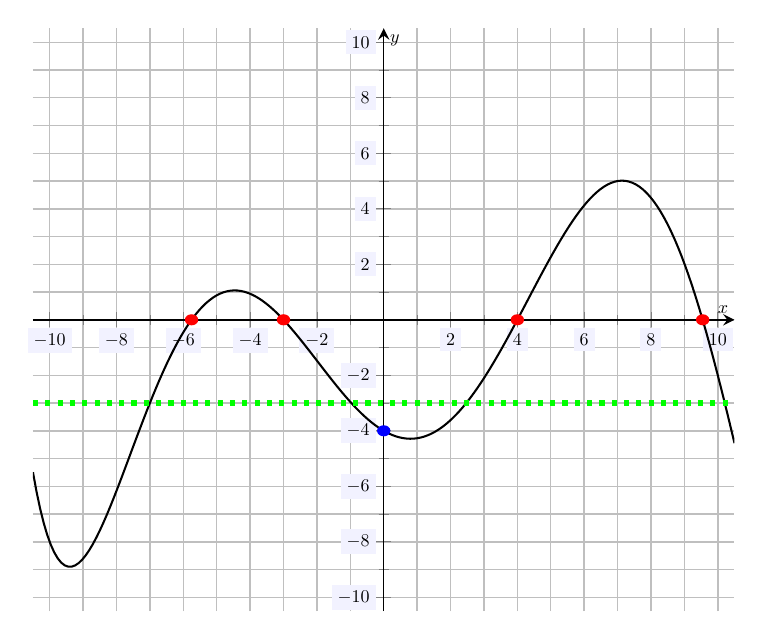
\begin{tikzpicture}[scale=1.3,every node/.style={scale=0.5}]
	\begin{axis}[
	grid=both,
	axis lines=middle,
	ticklabel style={fill=blue!5!white},
	xmin= -10.5, xmax=10.5,
	ymin= -10.5, ymax=10.5,
	xtick={-10,-8,-6,-4,-2,0,2,4,6,8,10},
	ytick={-10,-8,-6,-4,-2,0,2,4,6,8,10},
	minor tick = {-10,-9,...,10},
	xlabel=\(x\),ylabel=\(y\),
	]
	\addplot[line width= 0.02cm,samples=200,domain= -10.5:10.5] ({x},{-4. - 0.695759*x + 0.394934*x^2 + 0.0411407*x^3 - 0.00782987*x^4 - 0.000311831*x^5 + 0.0000378053*x^6}); 
	
	\draw[fill=blue,draw=none] (0,-4) circle (0.2);
	\draw[fill=red,draw=none] (-5.75251,0) circle (0.2);
	\draw[fill=red,draw=none] (-3,0) circle (0.2);
	\draw[fill=red,draw=none] (4,0) circle (0.2);
	\draw[fill=red,draw=none] (9.54717,0) circle (0.2);
	
	\draw[green,dotted,line width=0.05cm] (-10.5,-3) -- (10.5,-3);
	\end{axis}
	\end{tikzpicture}
	}
	\] 
Using the plot above, answer the following:
	\begin{enumerate}[(a)]
	\item Compute $\phi(9)$.
	\item Find the $y$-intercept for $\phi(x)$. 
	\item Find the $x$-intercepts for $\phi(x)$. 	
	\item As accurately as possible, compute the preimage of $-3$, i.e. $\phi^{-1}(-3)$. 
	\item Explain why (d) implies that $\phi$ does not have an inverse function. 
	\end{enumerate} \pspace

\sol 
\begin{enumerate}[(a)]
\item Because the plot contains the point $(9, 2)$, we can see that $\phi(9)= 2$. \pspace

\item The $y$-intercept is where the relation intersects the $y$-axis. We can see from the plot, shown in blue, that the $y$-intercept is the point $(0, -4)$, i.e. the $y$-intercept is $-4$. \pspace

\item The $x$-intercept(s) are the point(s) where the relation intersects the $x$-axis. We can see from the plot, shown in red, that the $x$-intercepts are $(-5.75251, 0)$, $(-3, 0)$, $(4, 0)$, and $(9.54717, 0)$, i.e. the $x$-intercepts are $-5.75251, -3, 4, 9.54717$. 

\item The value(s) of $\phi^{-1}(-3)$ are the $x$-values such that $\phi(x)= -3$. Graphically, these are $x$-values of the points on the curve that intersect the line $y= -3$, shown in green in the plot. Examining the plot, we can see that these are $-7$, $-0.968256$, $2.47042$, and $10.2091$, i.e. $\phi^{-1}(3)= \{ -7, -0.968256, 2.47042, 10.2091 \}$. 

\item We can see that the horizontal line at $y= -3$ intersects $\phi(x)$ more than once. Therefore, $\phi$ fails the horizontal line test. Therefore, $\phi$ does not have an inverse function. Alternatively, from (d), we see that $\phi^{-1}(-3)$ cannot be well-defined because there are 4 possible values for $\phi^{-1}$ as a function. 
\end{enumerate}


\end{document}